\documentclass[output=paper,newtxmath,modfonts,nonflat,draftmode]{langsci/langscibook} 
\author{Aurelie Takam\affiliation{Department of African Languages and Linguistics, University of Yaoundé\newline Department of French studies, York University}}
\title{Toward a better understanding of speech-language disorders in African countries: The case of speech sound disorders in Cameroon}
\abstract{Child speech and language disorders are not well known in many African countries. The aim of this study was to analyze speech sound disorders in Cameroon in order to encourage the rehabilitation of language disorders in general in the public health system. From a sample of 1127 children, 6\% of children presented with speech sound disorders including speech delays, articulation and phonological disorders. Boys were more affected than girls. Complex syllables and fricatives sounds were the most impaired while omission and substitution were the most frequent errors. }

\IfFileExists{../localcommands.tex}{%hack to check whether this is being compiled as part of a collection or standalone
  % add all extra packages you need to load to this file  
\usepackage{tabularx} 

%%%%%%%%%%%%%%%%%%%%%%%%%%%%%%%%%%%%%%%%%%%%%%%%%%%%
%%%                                              %%%
%%%           Examples                           %%%
%%%                                              %%%
%%%%%%%%%%%%%%%%%%%%%%%%%%%%%%%%%%%%%%%%%%%%%%%%%%%% 
%% to add additional information to the right of examples, uncomment the following line
% \usepackage{jambox}
%% if you want the source line of examples to be in italics, uncomment the following line
% \renewcommand{\exfont}{\itshape}
% \usepackage{lipsum}
% \usepackage[normalem]{ulem}
\usepackage{tikz}
\usepackage{tikz-qtree}
\usepackage{tikz-qtree-compat}
\usepackage{tabularx}
\usepackage{verbatim}
\usepackage{pifont}    %for pointing hand, checkmarks, crosses
\usepackage{tipa}
\usepackage{amssymb}
\usepackage{amsmath}
\usepackage{subcaption}
\usepackage{csquotes}
\usepackage{multirow}
\usepackage{multicol}
\usepackage{outlines} 
%\usepackage{wrapfig}
\usepackage{enumitem}
\usepackage{rotating}  
%\usepackage{ling-macros-custom}
\usepackage{stmaryrd}
%\usepackage{qtree}
\usepackage{./langsci/styles/langsci-optional}
\usepackage{./langsci/styles/langsci-lgr}
\usepackage{hhline}
\usepackage{langsci-gb4e}
\usepackage[linguistics]{forest}
 



   
\newcommand{\mc}[1]{\textsc{#1}}	% morpheme glossing as small caps: does not clash with fontspec
\def\Id#1{\vskip-.cm\hskip.01cm\vtop{#1}} % for controlling where the example breaks onto the next line


\setlength{\emergencystretch}{2pt}
\newcolumntype{s}{>{\hsize=.5\hsize}X}
\newcolumntype{m}{>{\hsize=.25\hsize}X}


 

%makes subscripts
\newcommand{\sub}[1]{\textsubscript{#1}}
\newcommand{\tikzmark}[1]{\tikz[overlay,remember picture]\node(#1){};}

%draws normal arrow
\newcommand*{\DrawArrow}[3][]{%
	\begin{tikzpicture}[overlay,remember picture, >=latex']
	\draw[rounded corners, -latex,<-,semithick,#1]  (#2) -- ++(0,-1.2em)coordinate (a) -- 
	($(a-|#3)$) -- (#3);
	\end{tikzpicture}%
}

%draws dashed arrow
\newcommand*{\DrawXArrow}[3][]{%
    % #1 = draw options
    % #2 = left point
    % #3 = right point
    \begin{tikzpicture}[overlay,remember picture,>=latex']
       % \draw [-latex, #1] ($(#2)+(0.1em,0.5ex)$) to ($(#3)+(0,0.5ex)$);
		\draw[rounded corners, -latex,<-,semithick,#1]  (#2) -- ++(0,-1.2em)coordinate (a) -- 
		node%[font=\footnotesize]
		{\ding{56}}
		($(a-|#3)$) -- (#3);
    \end{tikzpicture}%
}% 

\newcommand*{\DrawArrowok}[4][]{%
	% #1 = draw options
	% #2 = left point
	% #3 = right point
	\begin{tikzpicture}[overlay,remember picture, >=latex']
	% \draw [-latex, #1] ($(#2)+(0.1em,0.5ex)$) to ($(#3)+(0,0.5ex)$);
	\draw[rounded corners, -latex,<-,semithick,#1]  (#2) -- ++(0,-1.2em)coordinate (a) -- 
	%node[below,font=\footnotesize]{#4} 
	node[midway,fill=white,font=\normalsize]{#4}
	($(a-|#3)$) -- (#3);
	\end{tikzpicture}%
}% 

\newcommand*{\DrawLXArrow}[3][]{%
	% #1 = draw options
	% #2 = left point
	% #3 = right point
	\begin{tikzpicture}[overlay,remember picture,>=latex']
	% \draw [-latex, #1] ($(#2)+(0.1em,0.5ex)$) to ($(#3)+(0,0.5ex)$);
	\draw[rounded corners, -latex,<-,semithick,#1]  (#2) -- ++(0,-1.8em)coordinate (a) -- 
	node%[font=\footnotesize]
	{\ding{56}}
	($(a-|#3)$) -- (#3);
	\end{tikzpicture}%
}% 
\usetikzlibrary{arrows,shapes,positioning,shadows,trees,calc}
\usetikzlibrary{decorations.text}

 
\newcommand{\all}[1]{\ensuremath{\forall #1}}

\newcommand{\bari}{\ipabar{\i}{.5ex}{1.1}{}{}} 

\let\oldemptyset\emptyset
\let\emptyset\varnothing
 


\usetikzlibrary{calc,positioning,tikzmark}

%hyman
\newcommand{\higr}[1]{{\color{red}#1}}
 
 
\definecolor{lsDOIGray}{cmyk}{0,0,0,0.45}

%newkirk
\newcommand{\ix}[1]{{\color{red}\textsubscript{#1}}} %probably i.nde.x
\newcommand{\ol}[1]{{\color{red}\textit{#1}}} %probably o.bject l.anguage
\newcommand{\alert}[1]{{\color{red}\textbf{#1}}}
\newenvironment{context}{\color{red}
\smallskip 

\scriptsize 
}{\color{black}\normalsize }
\newcommand{\m}[1]{{\color{red}\textsc{#1}}}
\newcommand{\den}[1]{{\color{red}#1}}
\newcommand{\type}[1]{{\color{red}#1}}
\newcommand{\denol}[1]{{\color{red}#1}}
\newcommand{\bex}{\ea}
\newcommand{\fex}{\z}
\newcommand{\set}{{\color{red} SET}}
 
\def\denotes#1{$\lbrack\!\lbrack${#1\/}$\rbrack\!\rbrack$}      % denotes
\newcommand{\citeNP}{\citealt}


\makeatletter
\let\thetitle\@title
\let\theauthor\@author 
\makeatother


\newcommand{\togglepaper}[1][0]{ 
  \bibliography{../localbibliography}
  \papernote{\scriptsize\normalfont
    \theauthor.
    \thetitle. 
    To appear in: 
    Samson Lotven,   Silvina Bongiovanni,   Phillip Weirich,   Robert Botne \&  Samuel Gyasi Obeng (eds.),  
    African linguistics across the disciplines: Selected papers from the 48th Annual Conference on African Linguistics 
    Berlin: Language Science Press. [preliminary page numbering]
  }
  \pagenumbering{roman}
  \setcounter{chapter}{#1}
  \addtocounter{chapter}{-1}
}

 
  \togglepaper[10]
}{}


 
\begin{document} 
\shorttitlerunninghead{Toward a better understanding of speech-language disorders in Africa}
\maketitle


\section{Introduction} %1. /

Language disorders are not well known in many sub-Saharan countries. Our review of the literature indicates only a few African countries such as Togo, Nigeria, Kenya and South Africa, where studies have been carried out to describe the actual situation of these disorders (e.g. \citealt{Van2016}; \citealt{Topouzkhanian2013}). This paper aims to contribute toward this effort of better understanding language disorders in African countries given their considerable impact on primary education. Language disorders are impairments that affect the human language faculty and appear through one or many linguistic components of the spoken and written language. It is now well known that children with one or more of these impairments are at risk for limited social achievement. Speech sound disorder (SSD) and literacy difficulties (i.e. reading and spelling problems) are the most frequent language disorders among children \citep{Ruscello1991}. Our study specifically concerns the first category which are difficulties in producing or using speech sounds, very often the consonants, without organic alteration (such as hearing loss or cleft palate). The general objective of this study is to analyze these disorders in Cameroon in order to encourage the rehabilitation of language disorders in the public health system. In fact, in Cameroon as in many Sub-Saharan countries, children are not screened neither referred for assessment of speech and language disorders during their third or fourth year as it is usual in Nord American countries for example. In what follows, we present the profile and prevalence of SSD in order to shed light on their main characteristics. 

\subsection{Profile and classification of SSD} %1.1 /

Examples~to illustrate some speech sound errors are given in \tabref{tab:takam:0}.

\begin{table}
\caption{Speech sound errors\label{tab:takam:0}}
\begin{tabularx}{\textwidth}{XXX}
\lsptoprule
{French} {word}  & {illustration} & {Error} {types}\\
\midrule
\textit{viande}  & [vjãd] → [bjãd] & Substitution \\
\textit{couscous}  & [kuskus] → [tutu] & substitution; omission\\
\textit{chaise}  & [ʃɛz] → [ʃɛ] & omission\\
\textit{table}  & [tabl] → [tab] & omission\\
\textit{chocolat}  & [ʃokola] → [kokola] & consonant harmony\\
\lspbottomrule
\end{tabularx}
\end{table}


The generic terminology for these disorders varies in the literature, but in this study, we use the term “speech sound disorder” (SSD) to include articulation disorders, phonological delays and phonological disorders. Articulation disorders are phonetic in nature. For example, a child can systematically replace a sound with another regardless of the syllabic context (see examples 1 and 2 above) while another may systematically omit it (as in example 2). These types of systematic errors indicate a phonetic difficulty to perform the movement required to produce a sound \citep{Fox2001}. Another child may exhibit phonological errors that are specific to younger children. Here, a child may assimilate or omit a sound in a specific context and correctly produce it in another (as in examples 3, 4 and 5 above). The persistence of these types of errors above the expected age results in phonological delay. Thus a delay of at least six months is significant for this purpose \citep{Dodd2013}. %This was originally Dodd2011 but I cannot find the reference for this. I think Dodd2011 was what was intended.
However, when phonological errors are different from phonological processes (normal errors in phonological development), they are considered as atypical phonological errors and can be consistent or inconsistent depending on whether the same error pops up often or occasionally \citep{Dodd2013}. Finally, a child may exhibit a systematic error on a sound and assimilate another sound, thus showing an overlap between articulation and phonological problems. Therefore, we use the term SSD to include both articulation and phonological problems and the likely overlap between them.

\subsection{Prevalence of SSD}  %1.2. /

There is a lack of consensus on the prevalence rate of SSD from one study to another, ranging between 23\% and 2\% from our literature review \cite{McKinnon2007, Shriberg1999, Fombonne1997, Beitchman1986, Enderby1986, Kirkpatrick1984, Silva1984, Silva1980, Peckman1980, Stevenson1976, Morley1972, Hull1971}, Chevrie,. This inconsistency could be explained by the diversity of social factors (different countries: USA, Australia, Canada, France, Great Britain) as well as differences in methodological approaches (cross-sectional or longitudinal study, random or non-random sampling, one or several age groups). However, there seems to be a decrease in the rate of prevalence with age, these speech disorders being more frequent in younger preschool-aged children compared to school-aged ones \citep{Morley1972}. This rate decrease can be explained by the fact that preschool children have not yet acquired the complete phonology of their language and tend to master the use of speech sounds between the ages of six and seven years for languages such as French (e.g. \citealt{Rvachew2013}). Similarly, since some speech disorders are phonological delays, they may evolve and some children can catch up without speech intervention and perform well in formal tests (e.g.\citealt{BishopEdmundson1987}). However, it is worth noting that this apparent catch up may be illusory as some children often have residual phonological processing impairments (e.g. \citealt{Stothard1998}). Furthermore, all studies have higher prevalence rates for boys than girls (e.g. \citealt{Shriberg1999}). Finally, regarding the impact of socioeconomic status (SES) on the prevalence of articulatory disorders, \citet{McKinnon2007} conducted a study with 10425 students in Australia and found no difference between SES groups. In conclusion, the main variables to be studied for the prevalence of SSD are the status of the spoken language, age and gender.

\section{Context} %2. /
\subsection{Sociolinguistic description}  %2.1. /
\label{sec:takam:2.1}
Like many sub-Saharan countries, Cameroon is a multilingual country where children are exposed to at least two languages in their environment. Generally, bilinguals are categorized according to several factors but the main ones in this study are the age and order of exposure to both languages and the social status of the two languages. Therefore, we limited our attention to early bilingual Cameroonian children who speak Ghɔmálá’ and French and who live in one of the following sociolinguistic contexts: either a dominant French milieu (urban area) or a dominant Ghɔmálá’ milieu (rural area). However, whatever the region, French is the main language used at school in Cameroon and children are enrolled in the nursery school system from age three. This diglossic categorization of languages is a general feature of the sociolinguistic context in Cameroon, where the Administrative Atlas of National Languages \citep{Breton1991} lists 248 languages. In addition to this diversity, French and English are the two official languages. Based on the national distribution of official languages there are officially two linguistic communities: the French-speaking community (covering eight of the 10 regions) and the English-speaking community (covering the two remaining regions). Only the French-speaking community was covered in this study. 

Generally, the social status of French varies between urban and rural areas. Because urban areas are multilingual, French is the dominant language and it is acquired from an early age. This is the case in Bafoussam, the urban area investigated, where children acquire French as first language with the presence of Ghɔmálá’, the major local language spoken, and other minority languages. Compared to urban areas, rural areas provide a more homogeneous sociolinguistic environment where children are exposed both to the local language and French, and their contact with French intensifies with start of kindergarten at age three. Here, the local language is the main instrument of communication especially in the family environment and French is primarily used outside the home, especially by young people. Therefore in rural areas, the use of the local language is socially dominant although French is dominant at school and for public services. This is the case of Bandjoun, the rural area investigated in this study, where Ghɔmálá’ and French are spoken and where the child’s contact with French intensifies with entry into kindergarten. 

\subsection{Ghɔmálá’ and French} %2.2. /

Ghɔmálá’ and French are the main languages spoken in the Mifi, Kounghi-Khi and Hauts Plateaux administrative divisions in the western region of Cameroon \citep{Breton1991}. Compared to French, Ghɔmálá’ is a tone language with three simple and two complex tones (see \citet{Nissim1981} for a detailed description of Ghɔmálá’ phonology). Classified as a Bamiléké language (one of the Bantu languages) only spoken in Cameroon \citep{Dieu1983}, Ghɔmálá’ is comprised of 18 dialectal varieties with mutual comprehension. However, the variety of Bandjoun (Ghɔmálá’ jo) is used as the standard reference \citep{Domche1991}. Thus, this study covers speakers of this variety. Regarding French, children are exposed both to standard French (FS) mainly at school and through television and radio, and to the variety of Cameroonian French (FC) spoken in the western region of Cameroon. Besides, the French pronunciation to which the child is exposed varies according to the education level of the speakers. The elite with a high education level makes greater use of FS, while uneducated or less educated parents speak more in the local FC \citep{Biloa2004}. This means that children are exposed to both varieties of French. 

Ghɔmálá’ and French share many consonants. The consonant system of FC is based on FS phonology, comprising stops and fricatives, labial /p, b, m, f, v/, apical /t, d, n, s, z, l/, palatal /ʃ, ʒ, ɲ/, velar /k, g/, uvular /ʁ/ and glides /w, ɥ, j/. The majority of these consonants are oral against only three nasal /m, n, ɲ/. However, due to language contact, the FC may also include the nasal velar /ŋ/, the glottal fricative /h/ and the glottal stop /ʔ/ (see \citet{Biloa2004} for a detailed description of FC). In addition to these phonemes, Ghɔmálá’ also has the affricated consonants /pf, bv, ʦ, ʣ, ʧ, ʤ/ and the velar fricative /ɤ/ \citep{Mba1995}. However the uvular /ʁ/ is underrepresented in Ghɔmálá’ \citep{Mba1995}. For this reason, and as reported by \citet{Biloa2004}, some Ghɔmálá’ speakers of French may exhibit one or more of the following interference signs: in the coda position, /ʁ/ may be omitted (resulting in vowel lengthening or shortening), replaced by a glottal or a velar stop (e.g. [aʁʒɑ] “money” pronounced [a:ʒɑ], [agʒɑ] or [aʔʒɑ]), or simply replaced by the apical [r]; in syllable initial, /ʁ/ may be replaced by the apical [r] or the lateral [l]; finally in the consonant group, /ʁ/ may be omitted. Adding to this variation in the use of the uvular /ʁ/, the phonological interference between French and Ghɔmálá’ also appears through a tendency to articulate the mute “e” in syllable final (e.g. [tablə] instead of [tabl] “table”). There may be other interference processes but the ones listed here are the most frequent characteristics of the local ‘accent’. 

Finally, the distribution of consonants in the syllable structure shows some similarities and differences between French and Ghɔmálá’. In Ghɔmálá’ all the consonants can appear in initial position except for the glottal stop /ʔ/, but only the stops /p, m, k, ŋ, ʔ/ can appear in final position. However in French, all the consonants, including the palatal glide /j/, appear in both positions but the labial glides /ɥ/ and /w/ don’t appear in final. Concerning the structure of consonant groups, in Ghɔmálá’ they only appear in initial position and can have from two (CC) to four (CCCC) consonants. CC structure can be nasal + stop (e.g. /ŋkáp/ “money”) or stops + /h/ (e.g. /phə/ “bag”), and CCC and CCCC structures are made of (nasal+) nasal+stop+glide (e.g. /ŋkwə/ “foot”; /mŋkwə/ “feet”), nasal+stop+ /h/ (e.g. /mphə/ “bags”) or nasal+nasal+stop (e.g. /mntǎp/ “shoes”) where the first nasal may be the plural morphem /m-/. These structures are completely different from French where consonant groups may appear in initial and final syllable positions, and be composed of two (CC) and even three (CCC) consonants. French CC are formed of fricative+stop (e.g. /staʒ/ “traineeship”), stop or fricative + liquid or glide (e.g. /tʁɛ/ “train”; /bwa/ “wood”; /tabl/ “table”), while CCC structure may be composed of liquid +stop+liquid (e.g. /aʁbʁ/ “tree”) or stop+liquid+glide (e.g. /plɥi/ “rain”).

\section{The study} %3. /
\subsection{Objectives} %3.1 /

Using a clinical linguistic approach, the general objective of this study is to analyze SSD among a population of Cameroonian bilingual children. Specifically, the study aims to assess the prevalence of these disorders in preschool- and school-aged children and to describe their profile based on these age groups; that is, from 4--8 years old, in order to develop an intervention strategy. Besides, we also considered the fact that, generally, four-year-old children already have a good knowledge of the consonant system of their language (e.g., \citealt{MacLeodEtAl2011}). However, as Cameroonian children are often exposed to two or more languages, it is necessary to distinguish normal developing children from children with SSD. Based on the literature about the differences between bilingual and monolingual language acquisition, we have developed a procedure accordingly, as there is still no normative language data for the population under study. Even though the analysis of French consonant acquisition reveals that children living in a French dominant area master their consonant system around the age of six \cite{Rvachew2013}, researchers often point out the difference in the developmental trend of bilinguals compared to monolinguals, and the impact of the interaction between languages in bilingual language acquisition \cite{Paradis2011}. Therefore in this study, we limited the analysis to the consonants that are common to the languages spoken – French and Ghɔmálá’ – in order to avoid all variations related to language dominance in the child’s environment. We also considered that some errors may be due to that environment. 

\subsection{Method} %3.2 /

\subsection{Participants}

This study is based on a sample of 1127 bilingual French-Ghɔmálá’ children aged 4--8 years, who attended eight schools (five elementary schools and three kindergartens) with French as the only language of instruction (see \sectref{sec:takam:2.1} above for details). At the time of the investigation these children had been attending school for at least one year. The constitution of this sample was determined by the schools that were chosen according to their location, size and accessibility. As it appears in \tabref{tab:takam:sample_description} below, his sample includes 54\% of children living in the rural areas of Bandjoun, a Ghɔmálá’-dominant locality, and 46\% in the urban areas of Bafoussam, a French-dominant locality. There were 49\% girls and 51\% boys. The distribution of these children by age was as follows: four-year-olds\,=\,10\% (117 children), five-year olds\,=\,22\% (254 children), six-year olds\,=\,25\% (279 children), seven-year olds\,=\,20\% (221 children) and eight-year olds\,=\,23\% (256 children).

\begin{table}
\caption{Description of the sample based on school level, gender and socio-linguistic context ($N=1127$ children)\todo[inline]{This table was transposed to better fit the page. Please approve or comment}}
% \begin{tabularx}{.8\textwidth}{lSS}
% \lsptoprule
% 	& {N} & {\%} \\
% \midrule
% \textbf{School level}\\
% \midrule
% \textit{Maternelle} (kindergarten) & {136}  & 12\\
% {SIL} (grade 1) & {518}  & 46 \\
% {CP} (grade 2) & {473}  & 42 \\
% 
% \tablevspace
% \textbf{Gender}  &  & \\
% \midrule
% {girls} & {553}  & 49 \\
% {boys} & {574}  & 51 \\
% 
% \tablevspace
% {\textbf{Sociolinguistic context}}   & \\
% \midrule
% {rural} & {606}  & 54 \\
% {urban} & {521}  & 46\\
% \midrule
% \textbf{{Total} } & {1127}  & {100} \\
% \lspbottomrule
% \end{tabularx}
\begin{tabular}{l *{8}{r}}
\lsptoprule
 & \multicolumn{3}{c}{School level} & \multicolumn{2}{c}{Gender} & \multicolumn{2}{p{\widthof{Sociolinguistic}}}{Sociolinguistic context}\\\cmidrule(lr){2-4}\cmidrule(lr){5-6}\cmidrule(lr){7-8}
 & \textit{Maternelle}\footnote{(kindergarten)} & SIL\footnote{(grade 1)} & CP\footnote{(grade 2)} & girls & boys& rural & urban & Total\\\midrule
 $N$  & 136 & 518 & 473 & 553 & 574 & 606 & 521 & 1127\\
 \% &  12 &  46 &  42 &  49 &  51 &  54 &  46 &  100\\
\lspbottomrule
\end{tabular}
\label{tab:takam:sample_description}
\end{table}

\subsection{Procedure}

To assess the children’s speech-sound performance, we followed the recommendations of speech-language therapists regarding the combination of informal and formal procedures so as to have a sample of connected speech, to elicit a set of single-word productions by picture- or object-naming and to assess sound production in a repetition test. We therefore used a procedure based on the one proposed by \citet{MaurinCherou1993} for French-speaking children. In so doing, we were able to generally evaluate each child’s speech comprehension as well. Data collection took place over two school years, one school year per area, and was realized by the author of this paper who speaks Ghɔmálá’ and French as first languages, in collaboration with a linguist specialized in applied linguistics who verified the API transcription, and an ORL specialist who performed the medical exam. Schools were also selected based on their location, size and geographic accessibility. Subsequently, administrative formalities were completed in order to obtain the necessary authorizations to have access to the selected schools (which report to the education department) on the one hand and the classrooms (which are the responsibility of school principals) on the other hand. There were four steps in the data collection process: the teachers’ training workshop, the preliminary screening, the language and speech assessment, and the ORL exam.

\begin{description}
\item[Teachers’ training workshop:] After classifying the children by age groups, their classes and teachers were then identified. Then an information session and a training workshop were organized with the teachers of the selected classes about the preliminary identification of children at risk of developing speech-language disorders. For this preliminary screening, we explained the following criteria to the teachers:

\begin{enumerate}
    \item The child who speaks poorly (errors in the pronunciation of sounds, syllables, words and sentence)
    \item The child whose language expression is difficult to understand
    \item The child who has difficulty hearing and/or understanding
    \item The child who understands after several repetitions
    \item the child who is agitated or violent in class or out of class
    \item the child who is taciturn and doesn’t speak in class or out of class
\end{enumerate}

We were assisted by a speech-language therapist for the preparation of this workshop. 

\item[Preliminary screening:] After the training, teachers were given three months to draw up a list of children who met at least one of these criteria. The children identified were then assessed on their language use and speech production. This procedure had the merit of having the screening done on the basis of what is accepted as normal to the local population. A total of 100 children were listed by the teachers.

\item [Oral language assessment:] This assessment was conducted in an informal setting while establishing contact with the child before the formal assessment of speech sound production. First, the child was asked to talk about his/her usual activities and/or to tell a short story. The connected speech sampling was done in Ghɔmálá’ and French (see Appendix 1 for the list of some Ghɔmálá’ words used by the children). We then conducted a short vocabulary comprehension test following Maurin-Cherou’s protocol using some items randomly chosen from the picture-naming test. The child had to show the image of the spoken word among four choices. All the children passed this test. This assessment took about 15 minutes and the connected speech was recorded using an audio tape recorder. 

\item[Speech sound assessment:] Each child was evaluated during one session using two speech tests administered by the author of this paper: a picture-naming test and a word repetition test all in French. The child was first asked to name each picture of the naming test. Then s/he was asked to repeat a list of words chosen based on the sounds and syllabic structures that were difficult in the first test. The assessment lasted between 40 and 45 minutes and it was also recorded.

\begin{itemize}
\item  \textbf{The} \textbf{picture-naming} \textbf{test} consisted of producing 64 words prompted by colour pictures depicting well-known objects chosen from the local environment (see Appendix 2 for the list of the 64 words and Appendix 3 for a sample of pictures used). For some words, we used the object itself (e.g., for the word "grain" we used a sample of mixed grains of rice, corn and beans). The test assessed consonants common to Ghɔmálá’ and French but French was mainly used as the language of assessment given its dominant status at school. However, an eight-year-old girl and a four-year-old boy said a few words in Ghɔmálá’, in which case s/he had to repeat after the examiner. Each consonant appeared in different syllable positions except for the fricative [v]. The glides [w] and [j] mainly appeared in the consonant group. Other structures evaluated consisted of consonant+liquid, and the syllabic structures V, VC, CV, CVC. The children were able to name all the images as they reflected realities of their daily lives.
\item  \textbf{The} \textbf{repetition} \textbf{test} assessed the impaired consonants in different positions. The child had to repeat the word clearly articulated by the examiner.
\end{itemize}

\item[Oto-Rhino-Laryngology (or ORL) exam:] Only children identified as having SSD benefited from an ORL exam. The exams were conducted by a specialist in each of the target schools to evaluate the anatomical and physiological auditory system as well as the oral and respiratory system. Given that none of the screened children had organic disorders that could affect speech sound production (e.g. Hearing loss), in this study we present only the results of the speech sound assessment.
\end{description}

\subsection{Data analysis} %3.3 /

The identification of SSD was based on the analysis of consonants and syllabic structures from the connected speech sampled, the naming picture test and the repetition test. Each child’s production was collected using an individual form and recorded using an audio recorder. At the end of each day, for each child, data collected by the author of this paper were transcribed using the IPA and verified by an applied linguist. Speech disorders were identified by analyzing the child’s pronunciation based on expectations given his/her age. This was based on the consonant acquisition of 127 four-to-five-year-old French-speaking Cameroonian children living in a multilingual environment (Takam, in press). Generally, the results of this preliminary study showed no significant difference between the age groups (four-year-olds and five-year-olds): at least 90\% of the children were able to accurately produce the consonants [p, b, m, n, ɲ, j, f, s, v, k, d, ʒ, ʁ, w, z], around 80\% the fricative [ʃ] and only 60\% the lateral [l]. In the current study, errors were analyzed to determine the phonological processes classified as substitution, assimilation, omission, addition or metathesis as presented in the theoretical framework summarized in \tabref{tab:takam:2} below. 

\begin{table}
\caption{Classification of speech errors by structure (sound and syllable)}
\begin{tabularx}{\textwidth}{llQ}
\lsptoprule
{Structure}  & {Error}  & {Phonological} {process} {leading} {to} {the…}\\
\midrule
Sound & Substitution & replacement of a difficult sound by another causing a change in point or mode of articulation\\
\tablevspace
& Distortion & rough articulation producing a false noise\\
\tablevspace
& Assimilation & replacement of a sound which becomes like a nearby sound (sounds harmony)\\
\tablevspace
& Metathesis & position change of one or more sounds in the word\\
\tablevspace
Syllable & Omission & erasing of a sound\\
\tablevspace
& Addition & vocalic or consonantal addition\\
\tablevspace
& Metathesis & position change of one or more sounds in the word\\
\lspbottomrule
\end{tabularx}
\label{tab:takam:2}
\end{table}

\subsection{Result}  %3.4 /

\subsubsection{Prevalence rate}

Following the preliminary screening, 100 children were listed as presenting at least one of the criteria. At the end of the assessment, 32 children were excluded from this sample because they did not present any of the speech errors above (see table 2). Finally, 68 children presented with SSD in the form of phonetic disorders, phonological delays or phonological disorders, which represents a prevalence rate of about 6\% of the 1127 children in the population studied. Tables 3 and 4 below present this prevalence by gender, sociolinguistic context, school level and age group. There was a significant difference in prevalence rates by gender with 4.5\% of girls compared to 7.5\% of boys [$\chi^2 =  (1, N=1127) = 4.38, p=0.03$] and a ratio of 3.2. The prevalence rates by school level were also significantly different between kindergarten (8.8\%) and grade 1 pupils (7.5\%) on the one hand, and grade 2 pupils (3.6\%) on the other [$\chi^2 =  (2, N=1127) = 8.88, p=0.01$]. However, the percentage by age [$\chi^2 =  (4, N=1127) = 1.04, p=0.90$] and by sociolinguistic context [$\chi^2 =  (1, N=1127) = 0.37, p=0.54$] were not significantly different. 

\begin{table}
\caption{Prevalence rate by gender, sociolinguistic context and school level. $N$\,=\,general population; n\,=\,children with speech disorders; Mat\,=\,kindergarten (4--5 years); SIL\,=\,grade 1 (5--6 years); CP\,=\,grade 2 (6--8 years)}
\begin{tabularx}{.9\textwidth}{X *{8}{S[table-format=3.1]}}
\lsptoprule
& \multicolumn{2}{c}{Gender}  & \multicolumn{2}{p{\widthof{Sociolinguistic}}}{Sociolinguistic context} & \multicolumn{3}{c}{School level} &  Total \\\cmidrule(lr){2-3}\cmidrule(lr){4-5}\cmidrule(lr){6-8}
& \multicolumn{1}{c}{ Girls } & \multicolumn{1}{c}{ Boys } & \multicolumn{1}{c}{ Rural } & \multicolumn{1}{c}{ Urban } & \multicolumn{1}{c}{ Mat } & \multicolumn{1}{c}{ SIL } & \multicolumn{1}{c}{\textit{CP}} &  \\
\midrule 
 $N$ & 553 & 574 & 606 & 521 & 136 & 518 & 473 & \bfseries 1127\\
 $n$ & 25 & 43 & 39 & 29 & 12 & 39 & 17 & \bfseries 68\\
 \% & 4.5 & 7.5 & 6.4 & 5.6 & 8.8 & 7.5 & 3.6 & 6.0\\
\lspbottomrule
\end{tabularx}
\label{tab:takam:3}
\end{table}

\begin{table}
\caption{Prevalence rate by age groups}
\begin{tabularx}{.9\textwidth}{XSSSSS}
\lsptoprule
& \multicolumn{1}{c}{4 years} &  \multicolumn{1}{c}{5 years} &  \multicolumn{1}{c}{6 years} &  \multicolumn{1}{c}{7 years} &  \multicolumn{1}{c}{8 years}\\
\midrule
$N$  & 117 & 254 & 279 & 221 & 256\\
$n$  & 8 & 16 & 19 & 11 & 14\\
{\%} & 6.8 & 6.3 & 6.8 & 5.0 & 5.4\\
\lspbottomrule
\end{tabularx}
\label{tab:takam:4}
\end{table}


\subsubsection{Speech sound profile }%3.4.2

On a segmental level, {the analysis by age group showed some differences in the percentage accuracy of individual consonants} as presented in \tabref{tab:takam:5} below. There was a considerable decrease in the number of highly impaired consonants with age, but less variation in the consonants mode of articulation as they appear to be almost fricatives. {Generally, t}he sounds [l, ʁ] were impaired in all age groups while, on the contrary, the nasals [m, n] and the voiceless bilabial [p] were well used. Three categories of impaired consonants emerged following the classification of \citet{Shriberg1994}\footnote{\citet{Shriberg1994} distinguished three categories of consonants: the \textit{early-8} [m, b, j, n, w, d, p, h] with 100--80 percentage of correct production, the \textit{middle-8} [t, ŋ, k, g, f, v, ʧ, ʤ] with 70--30\%, and the \textit{late-8} [ʃ, θ, s, z, ð, l, r, ʒ], with less than 20\% frequency of correct use.}. Consonants [s, ʃ, z, l, ʁ] were the most impaired with more than 30\% of the children concerned, followed by the velars [k, g] with 10--30\% of children, and finally the sounds [v, ɲ, f, j, w, ɥ, b, t, d, ʒ] which were impaired for less than 10\% of the children. 

\begin{table}
\caption{Impaired consonants by age group. Not impaired: 0\% of the children; Low frequency: consonants impaired for less than 10\% of the children; Medium frequency: for 10--30\%; High frequency: for more than 30\%}
\label{tab:takam:5}
\begin{tabularx}{\textwidth}{Q@{~} lQQl@{}}
\lsptoprule
 Age groups &  Not impaired &  Low &  Medium &  Highly \\
\midrule
4 years\newline (n=8) & p, m, n, ɲ, ɥ  & n/a & j, v, d, w, f, t, b, k & ʒ, g, s, z, ʃ, l, ʁ\\
\tablevspace
5 years (n=16) & p, m, n, v, j & ʒ, ɲ, d, w, f, t & ɥ, g, k, b, s & z, ʃ, l, ʁ\\
\tablevspace
6 years (n=19) & p, m, n, ʒ, v, b, ɲ, d & w, f, v, t & ɥ, g, k, ʃ & l, s, z, ʁ\\
\tablevspace
7 years (n=11) & p, m, n, ɲ, v, f, b & ɥ, k, ʒ & j, w, t, g, d, s, z & ʃ, l, ʁ\\
\tablevspace
8 years (n=14) & p, m, n, w, ʒ, ɥ & v, b, ɲ, f, j, t, d & g, k & s, ʃ, z, l, ʁ\\
\midrule 
4--8 years (n=68) & {p,} {m,} {n} & {ɲ,} {v,} {f,} {ɥ,} {ʒ,} {j,} {w,} {b,} {t,} {d} & {g,} {k} & {s,} {ʃ,} {z,} {l,} {ʁ}\\
\lspbottomrule
\end{tabularx}
\end{table}



As far as syllable structures were concerned (see \tabref{tab:takam:6}), the CVC structure was the most impaired in all age groups with a frequency of about 97\%. Interestingly, all eight-year-olds altered this structure against 87\% of four-year-olds. On the other hand, the use of the consonant groups was much more laborious for four-to-five-year-olds.

\begin{table}
\caption{Impaired syllable structures by age group}
\begin{tabularx}{\textwidth}{XSSSSSS}
\lsptoprule
    & \multicolumn{1}{c}{4 years} & \multicolumn{1}{c}{5 years} & \multicolumn{1}{c}{6 years} & \multicolumn{1}{c}{7 years} & \multicolumn{1}{c}{8 years} & \multicolumn{1}{c}{4--8 years}\\
\midrule
  $n$  & 8 & 8 & 8 & 8 & 8 & 8\\
 CV & 6.2 & 31.2 & 36.8 & 27.3 & 28.6 & 32.3\\
 VC & 75.0 & 37.5 & 57.9 & 27.3 & 35.7 & 52.9\\
 CC & 75.0 & 68.7 & 31.6 & 36.4 & 35.7 & 52.9\\
 CVC & 87.5 & 93.7 & 94.7 & 90.9 & 100 & 97.0\\
\lspbottomrule
\end{tabularx}
\label{tab:takam:6}
\end{table}


{Finally,} omission and substitution were the most prevalent error forms as shown in \tabref{tab:takam:7} below. The Chi-square analysis of the percentage of children by age groups for each error reveals no significant difference. However, for distortion errors, the z-test with adjustment of the values according to the Bonferroni method indicated significant higher prevalence rates for four-year-olds (88\%) and six-year-olds (80\%) compared to the three other age groups: five-year-olds (\textit{44\%}); seven-year-olds (\textit{64\%}) and eight-year-olds (50\%). \REF{ex:takam:omission_errors} to \REF{ex:takam:assimilation_errors} below show detailed evaluations of these types of errors.

\begin{table}
\todo[inline]{no need to repeat $\chi^2=$}
\todo[inline]{what does =(4 mean?}
\caption{Frequency of speech sound errors by age (N=68 children)}
\label{tab:takam:7}
\begin{tabularx}{\textwidth}{lSSSS}
\lsptoprule
                & \multicolumn{2}{c}{4--8 years} & \multicolumn{1}{c}{$\chi^2(4, N=68)$} & \multicolumn{1}{c}{$p$}\\
\textbf{Errors} & \multicolumn{1}{c}{$n$} & \multicolumn{1}{c}{\%} & \\
\midrule
{O}mission     & 68 & 100    & 5.26 & .26\\
{S}ubstitution & 61 & 89.7   & 4.36 & .36\\
{D}istortion   & 43 & 63.2   & 7.12 & .10\\
Addition       & 32 & 44.1   & 5.69 & .22\\
Assimilation   & 22 & 32.4   & 4.28 & .37\\
\lspbottomrule
\end{tabularx}
\end{table}


Beginning with forms of omission, all the children revealed at least one of the following: syllable initial and final consonant omission, omission of an entire syllable, simplification of consonant groups and complex syllabic structures (see \REF{ex:takam:omission_errors} below for examples). Final consonant omission was the most frequent form regardless of age (approximately 93\% of the children), followed by the simplification of consonant groups (about 65\% of the children) and the omission of syllable initial consonants (about 43\% of the children). 

%\begin{table}
%\caption{Omission errors}

%\begin{tabularx}{\textwidth}{X}
%\lsptoprule

%\textit{-syllable final consonant omission}\\
%(ardoise) [aʁ-dwaz] > [a-dwaz] $\rightarrow$ V\textbf{C} > V\\
%(couscous) [kuskus] > [ku-kus] $\rightarrow$ CV\textbf{C} > CV\\
%\midrule
%\textit{-syllable initial consonant omission}\\
%(parapluie) [pa-\textbf{ʁ}a-plɥi] > [pa:-plɥi] $\rightarrow$ CV>V\textbf{:}\\
%(arachide) /a-\textbf{ʁ}a-ʃid/ >  /a:-ʃid/ $\rightarrow$ CV>V\textbf{:}\\
%\midrule
%\textit{-simplification of consonants group}\\
%(crayon) [kʁe-jɔ] > [ki-jɔ] $\rightarrow$ C\textbf{C}V > CV\\
%(table)  [tabl] > [tab] \biberror{[F0E0?]} CVC\textbf{C} > CVC\\
%\midrule
%\textit{-syllable omission}\\
%(nourriture) [nu-ʁ\textbf{i}-tyʁ] > [nu:-ty:] $\rightarrow$ CV\\
%(télévision) [te-le-\textbf{vi}-zjɔ] > [te-le-sjɔ] $\rightarrow$ CV\\
%\midrule
%\textit{-simplification of complex syllable structures}\\ 
%(arbre)  [a:ʁbʁ] > [a:b] $\rightarrow$ V\textbf{C}C\textbf{C} > VC\\
%(parapluie) [pa-ʁa-plɥi] > [pa-ha-ply] $\rightarrow$ CC\textbf{C}V > CCV\\
%\lspbottomrule
%\end{tabularx}
%\label{tab:takam:8}
%\end{table}

\ea Omission errors \label{ex:takam:omission_errors}
\ea\relax {syllable final consonant omission}\\
(ardoise) [aʁ-dwaz] > [a-dwaz] $\rightarrow$ V\textbf{C} > V\\
(couscous) [kuskus] > [ku-kus] $\rightarrow$ CV\textbf{C} > CV\\

\ex\relax {syllable initial consonant omission}\\
(parapluie) [pa-\textbf{ʁ}a-plɥi] > [pa:-plɥi] $\rightarrow$ CV>V\textbf{:}\\
(arachide) /a-\textbf{ʁ}a-ʃid/ >  /a:-ʃid/ $\rightarrow$ CV>V\textbf{:}\\

\ex\relax {simplification of consonants group}\\
(crayon) [kʁe-jɔ] > [ki-jɔ] $\rightarrow$ C\textbf{C}V > CV\\
(table)  [tabl] > [tab] $\rightarrow$ CVC\textbf{C} > CVC\\

\ex\relax {syllable omission}\\
(nourriture) [nu-ʁ\textbf{i}-tyʁ] > [nu:-ty:] $\rightarrow$ CV\\
(télévision) [te-le-\textbf{vi}-zjɔ] > [te-le-sjɔ] $\rightarrow$ CV\\

\ex\relax {simplification of complex syllable structures}\\ 
(arbre)  [a:ʁbʁ] > [a:b] $\rightarrow$ V\textbf{C}C\textbf{C} > VC\\
(parapluie) [pa-ʁa-plɥi] > [pa-ha-ply] $\rightarrow$ CC\textbf{C}V > CCV\\
\z
\z

Substitution errors appeared as a systematic or an inconsistent replacement of a consonant leading to a variety of errors such as fronting, backing, stopping, gliding and devoicing (see \REF{ex:takam:substitution_errors} below). In general, the substitution of [ʃ, ʒ] to [s, z] was the most frequent with a 68\% prevalence rate, followed by backing, gliding and fronting errors with a 40--60\% prevalence rate. Apart from devoicing (15\% of the children) the other forms listed had prevalence rates less than 10\%.

\ea Substitution errors \label{ex:takam:substitution_errors}
\ea \relax {fronting}\\
(couscous) [kuskus] > [tutu] $\rightarrow$ [k] > [t]\\
(chat) [ʃa] > [sa] $\rightarrow$ [ʃ] > [s]\\

\ex\relax {substitution} {of} {[l]} {to} {[j]}\\
 (crayon) [kʁejɔ] > [kʁelɔ] $\rightarrow$ [j] > [l]\\ 
(bouteille) [butɛj] > [butɛl] $\rightarrow$ [j] > [l]\\

\ex\relax {backing}: \\
(tasse) [tas] > [kas] $\rightarrow$ [t] > [k]\\
(train) [tʁɛ] > [kʁɛ] $\rightarrow$ [t] > [k]\\

\ex\relax {substitution of [ʃ,ʒ] to [s,z]:}\\ 
(tasse) [tas] > [taʃ] $\rightarrow$ [s] > [ʃ]\\
(maison) [mɛzɔ] > [mɛʒɔ] $\rightarrow$ [z] > [ʒ] \\

\ex\relax {stopping}: \\
(savon) [savɔ] > [tavɔ]] $\rightarrow$ [s] > [t]\\ 
(carte) [kaʁt] > [kaktə] $\rightarrow$ [ʁ] > [k]\\

\ex\relax {substitution of [l] to [ʁ]}\\
(robe) [ʁɔb] > [lɔb] $\rightarrow$ [ʁ] > [l]\\ 
(orange) [oʁãʒ] > [olãʒ] $\rightarrow$ [ʁ] > [l]\\

\ex\relax {gliding}:\\
(fleur) [fløʁ] > [fwøʁ] $\rightarrow$ [l] > [w]\\ 
(ballon) [balɔ] > [bajɔ] $\rightarrow$ [l] > [j]\\

\ex\relax {substitution of vowel to glide}\\
(parapluie) [paʁaplɥi] > [palaply] $\rightarrow$ [ɥ]> [y]\\

\ex\relax {Devoicing}:\\
(doigt) [dwa] >[twa] $\rightarrow$ [d]> [t]\\
\z
\z

%\begin{table}
%\caption{Substitution errors}

%\begin{tabularx}{\textwidth}{XX}
%\lsptoprule
%\textit{fronting}: 
%(couscous) [kuskus] > [tutu] \biberror{[F0E0?]}[k] > [t] 
%(chat) [ʃa] > [sa] \biberror{[F0E0?]} [ʃ] > [s] & \textit{substitution} \textit{of} \textit{[l]} \textit{to} \textit{[j]}
%(crayon) [kʁejɔ] > [kʁelɔ] \biberror{[F0E0?]} [j] > [l] 
%(bouteille) [butɛj] > [butɛl] \biberror{[F0E0?]} [j] > [l]\\
%\textit{backing}: 
%(tasse) [tas] > [kas] \biberror{[F0E0?]} [t] > [k]
%(train) [tʁɛ] > [kʁɛ] \biberror{[F0E0?]} [t] > [k] & \textit{substitution} \textit{of} \textit{[ʃ,} \textit{ʒ]} \textit{to} \textit{[s,} \textit{z]:} 
%(tasse) [tas] > [taʃ] \biberror{[F0E0?]} [s] > [ʃ] 
%(maison) [mɛzɔ] > [mɛʒɔ] \biberror{[F0E0?]} [z] > [ʒ] \\
%\textit{stopping}: 
%(savon) [savɔ] > [tavɔ]] \biberror{[F0E0?]} [s] > [t] 
%(carte) [kaʁt] > [kaktə] \biberror{[F0E0?]} [ʁ] > [k] & \textit{substitution} \textit{of} \textit{[l]} \textit{to} [ʁ]
%(robe) [ʁɔb] > [lɔb] \biberror{[F0E0?]} [ʁ] > [l] 
%(orange) [oʁãʒ] > [olãʒ] \biberror{[F0E0?]} [ʁ] > [l]\\
%\textit{gliding}: 
%(fleur) [fløʁ] > [fwøʁ] \biberror{[F0E0?]} [l] > [w] 
%(ballon) [balɔ] > [bajɔ] \biberror{[F0E0?]} [l] > [j] & \textit{substitution} \textit{of} \textit{vowel} \textit{to} \textit{glide} %(parapluie) [paʁaplɥi] > [palaply]\biberror{[F0E0?]}[ɥ]> [y]
%\textit{Devoicing:} (doigt) [dwa] >[twa] \biberror{[F0E0?]} [d]> [t]\\
%\lspbottomrule
%\end{tabularx}
%\label{tab:takam:9}
%\end{table}


Regarding the errors classified as distortions, about 63\% of the children glottalized /ʁ/ and only 12\% of them also distorted the apical /t/ and the velar /k/ in syllable initial. It is worth recalling that in this study, distortion errors were neither a substitution nor an assimilation but an approximate production of a segment. Based on \tabref{tab:takam:2} above, the Chi-square analysis revealed no significant difference by age group [$\chi^2 = (4, N=68) = 7.12, p=0.10$]. However, the z-test with adjustment of the values according to the Bonferroni method indicated higher prevalence rates for four-year-olds (88\%) and six-year-olds (80\%) compared to the three other age groups: five-year-olds (\textit{44\%}); seven-year-olds (\textit{64\%}) and eight-year-olds (50\%). \REF{ex:takam:distortion_errors} below shows examples of distortion errors observed. 

\ea Forms of distortion errors \label{ex:takam:distortion_errors}
\ea Distortion of [t]:\\
(pantalon) [pãtalɔ] > [pãt\textsuperscript{h}alɔ] $\rightarrow$ [t] > [t\textsuperscript{h}]\\
(voiture) [vwatyʁ] > [vwat\textsuperscript{h}y] $\rightarrow$ [t] > [t\textsuperscript{h}]\\
\ex Distortion of [k]:\\ 
(car) [kaʁ] > [k\textsuperscript{h}a] $\rightarrow$ [k] > [k\textsuperscript{h}]\\
(crayon) [kʁejɔ] > [k\textsuperscript{h}ejɔ] $\rightarrow$ [k] > [k\textsuperscript{h}]\\
\ex Distortion of [ʁ]:\\
(radio) [ʁadjo] > [hadjo] $\rightarrow$ [ʁ] > [h]\\
(robe) [ʁɔb] > [hɔb] $\rightarrow$ [ʁ] > [h] \\
\z
\z

%\begin{table}
%\caption{Forms of distortion errors}
%\begin{tabularx}{\textwidth}{XX}
%\lsptoprule
%\multicolumn{1}{c}{- distortion of [t]:
%(pantalon) [pãtalɔ] > [pãt\textsuperscript{h}alɔ] / [t] > [t\textsuperscript{h}] (voiture) [vwatyʁ] > [vwat\textsuperscript{h}y] / [t] > [t\textsuperscript{h}]} & - distortion of [k] 
%(car) [kaʁ] > [k\textsuperscript{h}a] \biberror{[F0E0?]} [k] > [k\textsuperscript{h}] 
%(crayon) [kʁejɔ] > [k\textsuperscript{h}ejɔ] \biberror{[F0E0?]} [k] > [k\textsuperscript{h}] \\
%\multicolumn{2}{c}{- distortion of [ʁ]: (radio) [ʁadjo] > [hadjo] \biberror{[F0E0?]}[ʁ] > [h]; (robe) [ʁɔb] > [hɔb] / [ʁ] > [h]} \\
%\lspbottomrule
%\end{tabularx}
%\label{tab:takam:10}
%\end{table}


Sound addition errors were present in about 44\% of the children. One form was the simplification of a complex syllable structure by adding an epenthetic vowel. It concerned about 15\% to 37\% of children between the ages of 6--8 years. The other form, the most prevalent, was the adding of a consonant at the beginning of words with vocalic attack. It affected all age groups. \REF{ex:takam:addition_errors} below illustrates these forms of errors.

\ea Addition errors \label{ex:takam:addition_errors}
\ea Vocalic addition (epenthesis)\\
    (fleur) [fløʁ] > [f\textbf{ə}-lø:] $\rightarrow$ CCVC > C\textbf{V}+CV\\
    (brosse) [bʁos] > [b\textbf{ə}-los] $\rightarrow$ CCVC > C\textbf{V}+CVC\\
\ex Consonant addition\\
    (ardoise) [aʁ-dwaz] > [\textbf{n}aʁ-dwaz] $\rightarrow$ VC > \textbf{C}VC\\
(hache) [aʃ] > [\textbf{ʁ}aʃ] $\rightarrow$ VC > \textbf{C}VC\\
\z
\z
%\begin{table}
%\caption{Addition errors}
%\begin{tabularx}{\textwidth}{XX}
%\lsptoprule
%vocalic addition (epenthesis)
%(fleur) [fløʁ] > [f\textbf{ə}-lø:] \biberror{[F0E0?]} CCVC > C\textbf{V}+CV 
%(brosse) [bʁos] > [b\textbf{ə}-los] \biberror{[F0E0?]} CCVC > C\textbf{V}+CVC & Consonant addition 
%(ardoise) [aʁ-dwaz] > [\textbf{n}aʁ-dwaz] \biberror{[F0E0?]} VC > \textbf{C}VC
%(hache) [aʃ] > [\textbf{ʁ}aʃ] \biberror{[F0E0?]} VC > \textbf{C}VC \\
%\lspbottomrule
%\end{tabularx}
%\label{tab:takam:11}
%\end{table}

Finally, assimilation errors appeared as regressive or progressive consonant harmony and consonant devoicing as shown in \REF{ex:takam:assimilation_errors} below. About 32\% of children presented one or more of these errors without any significant difference between groups. Regressive assimilation of /ʃ/ and devoicing errors were the main forms observed.

\ea Assimilation errors \label{ex:takam:assimilation_errors}
\ea Progressive assimilation\\
    (pantalon)  [pãtalɔ] > [pãpalɔ] $\rightarrow$ [t] > [p]\\
\ex Regressive assimilation\\
    (chemise) [ʃəmiz] > [səmiz] $\rightarrow$ [ʃ] > [s]\\
    (chapeau) [ʃapo] > [papo] $\rightarrow$ [ʃ] > [p]\\
    (fourchette) [fuʁʃɛt] > [fuʁsɛt] $\rightarrow$ [ʃ] > [s]\\
    (chocolat) [ʃokola] > [kokola] $\rightarrow$ [ʃ] > [k]\\ 
    (arachide) [aʁaʃid] > [aʁatid] $\rightarrow$  [ʃ] > [t]\\
\ex Devoicing\\
    (gâteau) [gato] > [kato] $\rightarrow$ [g] > [k]\\
    (table) [tabl] > [tap] $\rightarrow$ [b] > [p]\\
\z
\z
%\begin{table}
%\caption{Assimilation errors}

%\begin{tabularx}{\textwidth}{XX}
%\lsptoprule

%Progressive assimilation: & Regressive assimilation:\\
%(\textit{pantalon}) [pãtalɔ] > [pãpalɔ] \biberror{[F0E0?]} [t] > [p] & (\textit{chemise}) [ʃəmiz] > [səmiz] \biberror{[F0E0?]} [ʃ] > [s] \\
%devoicing: 
%(\textit{gâ}\textit{teau}) [gato] > [kato] \biberror{[F0E0?]} [g] > [k]
%(\textit{table}) [tabl] > [tap] \biberror{[F0E0?]} [b] > [p] & (\textit{chapeau}) [ʃapo] > [papo] \biberror{[F0E0?]} [ʃ] > [p]
%(\textit{fourchette}) [fuʁʃɛt] > [fuʁsɛt] \biberror{[F0E0?]} [ʃ] > [s] (\textit{chocolat}) [ʃokola] > [kokola] \biberror{[F0E0?]} [ʃ] > [k] 
%(\textit{arachide}) [aʁaʃid] > [aʁatid] \biberror{[F0E0?]}  [ʃ] > [t]\\
%\lspbottomrule
%\end{tabularx}
%\label{tab:takam:12}
%\end{table}


\subsubsection{Discussion} %3.5 /

This study was aimed at assessing SSD from a representative quasi-random sample of 1127 bilingual Cameroonian children aged four to eight years and living in two Ghɔmálá’-French environments (rural and urban). The prevalence rate of 6\% obtained in this study is comparable to the rate of 7.8\% obtained by \citet{Fombonne1997} among French children between four and 16 years of age. In general, \citet{Kirkpatrick1984} place this prevalence between 4\% and 6\%. These studies indicated a higher prevalence for boys compared to girls as was also the case in the present study. This difference is not yet explained in the literature. However, this discrepancy is also observed in regular language development as it is well admitted that girls generally develop speech and language faster than boys. However, this speed difference is significant, up to 30 months \citep{Eriksson2012}. 

Regarding the differences related to school level, it is important to note that most children with SSD were more in kindergarten and grade 1 (SIL). Many of the first-grade children in this study had failed to progress to the second grade (CP).These results can be interpreted as evidence that SSD is a handicap to children's academic performance. Several studies have linked SSD to children's education and it is now well recognized that they can give rise to learning disabilities such as difficulty learning written language graphemes (e.g.~\citealt{Rvachew2007}). One explanation is that SSD is often related to a phonological awareness deficit which plays a significant role in written language learning. This causal relation is mainly determined by the severity of the disorders profile regarding types of errors (e.g. omission) and error pattern, whether they are typical or atypical among normal developing children \cite{RvachewChiangEvans2007}. Omission errors are considered more severe than substitution as are atypical errors compared to typical ones.

Concerning the speech profile of the disorders in our sample, the main errors were omission and substitution without a significant difference between groups. Omission errors mainly occurred as final consonant omission and consonant group simplification, while the substitution of [ʃ, ʒ] to [s, z] was the most frequent with about 68\% of the children, followed by backing, gliding and fronting errors with a 40--60\% prevalence rate. According to \citet{RvachewChiangEvans2007} and \citet{Fox2001}, all these forms of errors are also typical to normal developing children. Consonants [s, ʃ, z, l, ʁ] and CVC syllables were the most impaired structures. These results are consistent with the literature both regarding type of errors (e.g.\citealt{Austin1997,Ruscello1991}) and impaired consonants (e.g. \citet{MaurinCherou1993} for French-speaking children; \citet{Shriberg1994} for English-speaking children). Besides, our analysis emphasized the importance of the syllabic structure including the lexical position and environment of consonants. Very few studies (e.g.~\citealt{RvachewChiangEvans2007}) have examined this aspect while assessment and intervention always include them in order to better evaluate speech difficulties (e.g. \citealt{MaurinCherou1993}). 

Regarding the impairment of [ʁ] in this study, all the children had difficulties with its use. This consonant is among the most frequent in French \citep{Peytard1970} while it is almost absent in Ghɔmálá’ \citep{Mba1995}. Some of the error forms reported here were the same as those observed in the sociolinguistic context of the children as described by \citet{Biloa2004}. However, the difficulties with this sound were not only due to language interference or input given that the errors were not always linked to the sociolinguistic context. In fact, several studies have reported difficulties with this consonant in different linguistic environments. In English (or native English) children, the apical [r] is usually substituted for the glide [w] in initial position \citep{Bowen2014}. As for monolingual Francophones, this is a sound frequently affected by SSD \cite{MaurinCherou1993}.

\subsection{Conclusion} %4. /

The objective of this study was to analyze child SSD in Cameroon in order to encourage the rehabilitation of language disorders in the public health system. Using a sample of 1127 bilingual children between the ages of four and eight years, the study determined the prevalence and speech profile of these disorders. In a nutshell, 6\% of the children presented with SSD without a significant difference between age groups and sociolinguistic context (rural and urban). However, boys were more affected than girls with a ratio of 3.2. On the phonic level, consonants [ʁ, l, s, z, ʃ] were the most impaired (with 30\% to 100\% of the children screened) and the most frequent errors were omission and substitution. On the syllabic level, complex structures in general and the CVC structure, in particular, were the most impaired with a frequency of more than 90\% followed by consonant groups with more than half of the children. The need for intervention no longer needs justification since these disorders have an impact both on individual and school performance. There are some limits to this study regarding the comorbidity of the speech disorders studied. None of the screened children had any difficulty understanding oral language. However, since we did not assess their language abilities (e.g., grammatical knowledge), it is possible that some of them may have a language delay.
 


\clearpage
\subsection{Appendix}
% \begin{table}
\subsubsection{A sample of Ghɔmálá’ words used (IPA)}

\begin{tabularx}{\textwidth}{XXX}
% \lsptoprule
/phə/ ‘bag’

/paʔ/ ‘house’

/bjɛ/ ‘groundnuts’

/mɔk/ ‘fire’

/nàm/ ‘sun’

/wâsi/ ‘watch’

/sɛdjə/ ‘broom’ & /bàp/ ‘meat’

/dàp/ ‘thread’

/nɔk/ ‘snake’

/sɔk/ ‘soap’

/ʧòʔ/ ‘hat’

/ŋkedé/ ‘banana’

/ʦə/ ‘cola nut’ & /saʔthə/   ‘comb’

/ŋwàʔɲə/ ‘book’

/ʤɔm/ ‘axe’

/bvʉ/ ‘dog’

/púsi/ ‘cat’

/ʣə/ ‘clothe’

/wɔktə/ ‘umbrella’\\
% \lspbottomrule
\end{tabularx}
% \end{table}


% \begin{table}
\subsubsection{List of the 64 words (in French) used for picture naming and word repetition tests }

\begin{tabularx}{\textwidth}{XXXX}
% \lsptoprule
\textit{ananas}

\textit{arachide}

\textit{arbre~}

\textit{ardoise}

\textit{assiette} 

\textit{avion} 

\textit{bague}

\textit{ballon}

\textit{banane}

\textit{blanc} 

\textit{bonbon~}

\textit{bouteille}

\textit{brosse} 

\textit{cahier}

\textit{autocar}

\textit{carte} & \textit{casque} 

\textit{chaise}

\textit{chapeau}

\textit{chat}

\textit{chaussure}

\textit{chemise}

\textit{couscous}

\textit{crayon}

\textit{doigt}

\textit{drap} 

\textit{fenêtre} 

\textit{feu}

\textit{fleur} 

\textit{fourchette}

\textit{gâteau}

\textit{gomme} & \textit{grains} 

\textit{hache}

\textit{huile}

\textit{journal}

\textit{livre} 

\textit{maison}

\textit{marmite}

\textit{montre} 

\textit{nourriture}

\textit{œuf}

\textit{oignon}

\textit{oiseau}

\textit{orange}

\textit{pantalon}

\textit{parapluie}

\textit{peigne} & \textit{pipe}

\textit{plantain~}

\textit{porte}

\textit{radio}

\textit{robe}

\textit{sac}

\textit{savon}

\textit{serpent}

\textit{soleil}

\textit{table}

\textit{tasse}

\textit{téléphone}

\textit{télévision}

\textit{train}

\textit{voiture}

\textit{yaourt}\\
% \lspbottomrule
\end{tabularx}
% \end{table}


\begin{figure}
\caption{A sample of pictures used for the naming test}

\begin{tabularx}{\textwidth}{XXXX}
% \lsptoprule

\includegraphics[width=.2\textwidth]{figures/takam-img1.png} & 
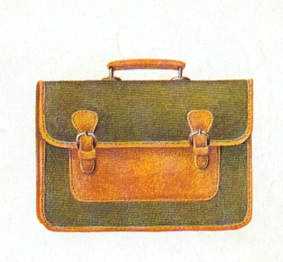
\includegraphics[width=.2\textwidth]{figures/takam-img2.png} & 

\includegraphics[width=.2\textwidth]{figures/takam-img3.png} & 
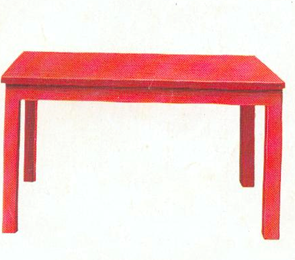
\includegraphics[width=.2\textwidth]{figures/takam-img4.png} \\
                       
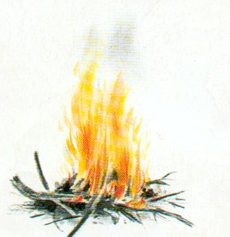
\includegraphics[width=.2\textwidth]{figures/takam-img5.png} & 
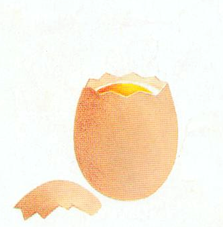
\includegraphics[width=.2\textwidth]{figures/takam-img6.png} & 
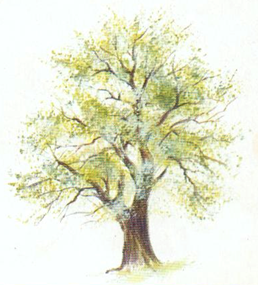
\includegraphics[width=.2\textwidth]{figures/takam-img7.png} & 
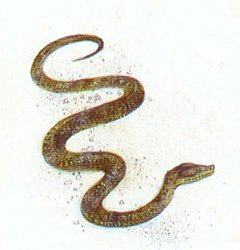
\includegraphics[width=.2\textwidth]{figures/takam-img8.png} \\
                       
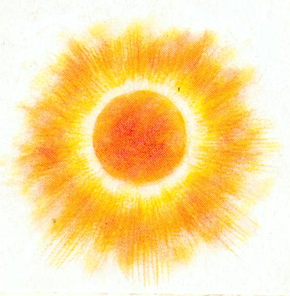
\includegraphics[width=.2\textwidth]{figures/takam-img9.png}  &
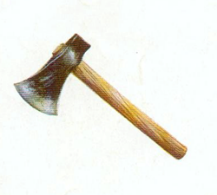
\includegraphics[width=.2\textwidth]{figures/takam-img10.png} & 
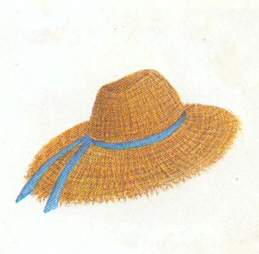
\includegraphics[width=.2\textwidth]{figures/takam-img11.png}  & 
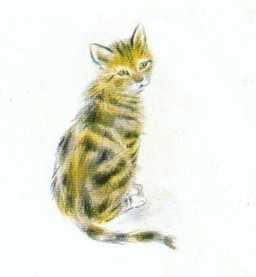
\includegraphics[width=.2\textwidth]{figures/takam-img12.png}\\
% \lspbottomrule
\end{tabularx}
\todo[inline]{copyright status of the pictures must be established}
\end{figure}

\begin{comment}%%move bib entries to  localbibliography.bib

@misc{Austin1997,
	author = {Austin, D.  and  Shriberg, L. D},
	number = {3},
	series = {Tech. Rep. No},
	title = {Lifespan reference data for ten measures of articulation competence using the Speech Disorders Classification System ({SD}{CS})},
	year = {1997}
}


@article{Beitchman1986,
	author = {Beitchman, J. H., Nair, R., Clegg, M.  and  Patel, P. G},
	journal = {Journal of Speech and Hearing Disorders},
	pages = {98--110},
	title = {Prevalence of speech and language disorders in five-year-old kindergarten children in the {Ottawa}-Carleton region},
	volume = {51},
	year = {1986}
}


@book{Biloa2004,
	address = {Bern, Berlin, Bruxelles, Frankfurt am Main, New York, Oxford & Wien},
	author = {Biloa, E.},
	publisher = {Peter Lang},
	title = {{La} {La}ngue Française au Cameroun: {{A}}nalyse linguistique et didactique. 2e edition},
	year = {2004}
}


@misc{Bowen2014,
	author = {Bowen, C},
	title = { Children's speech sound disorders. {{J}}ohn Wiley & Sons.},
	year = {2014}
}


@book{Breton.1991,
	address = {Paris},
	author = {Breton. R.  and  Fohtung, B.},
	publisher = {ACCT Cerdotola},
	title = {Atlas Administratif des Langues Nationales du Cameroun},
	year = {1991}
}


@book{Delattre1966,
	address = {La Haye},
	author = {Delattre, P.},
	publisher = {Mouton},
	title = {Studies in {French} and Comparative Phonetics},
	year = {1966}
}


@book{Dieu1983,
	address = {Paris, Yaoundé},
	author = {Dieu, M.  and  Renaud, P.},
	publisher = {ACCT, CERDOTOLA, DGRST},
	title = {Atlas Linguistique d’Afrique Centrale ({AL}{AC}) : {{S}}ituation linguistique en Afrique Centrale. {{I}}nventaire préliminaire: {{L}}e Cameroun},
	year = {1983}
}


@misc{Dodd2013,
	author = {Dodd, B},
	title = { Differential diagnosis and treatment of children with speech disorder. 2nd edition. {{J}}ohn Wiley & Sons.},
	year = {2013}
}


@book{Domche1991,
	address = {Yaoundé},
	author = {Domche, E.  and  Hatfield.},
	publisher = {SIL},
	title = {Enquète Sociolinguistique sur le Ghɔmálá’-Jo comme Dialecte de Référence Standard},
	year = {1991}
}


@article{Enderby1986,
	author = {Enderby, P.  and  Philipp, R},
	journal = {British Journal of Disorders of Communication},
	pages = {151--165},
	title = {Speech and language handicap: {{T}}oward knowing the size of the problem},
	volume = {21},
	year = {1986}
}


@article{Eriksson2012,
	author = {Eriksson, M., Marschik, P. B, Tulviste, T., Almgren, M., Pereira, M. P., Wehberg, S., Marjanoviˇc-Umek, L., Gayraud, F., Kovacevic, M.  and  Gallego, C},
	journal = {British Journal of Developmental Psychology},
	pages = {326–343},
	title = {Differences between girls and boys in emerging language skills: {{{E}}}vidence from 10 language communities},
	volume = {30},
	year = {2012}
}
%%%

@article{Fombonne1997,
	author = {Fombonne, E.  and  Vermeersh, S},
	journal = {Revue Epidémiologique de Santé Publique},
	pages = {107--115},
	title = {Les enfants de la cohorte {GA}{ZE}L: {{I}}I - Motifs des contacts avec le système médico-éducatif, par âge et sexe”},
	volume = {45},
	year = {1997}
}


@article{Fox2001,
	author = {Fox, A. V.,  and  Dodd, B},
	journal = {American Journal of Speech-Language Pathology},
	number = {3},
	pages = {291--307},
	title = {Phonologically disordered {German}-speaking children},
	volume = {10},
	year = {2001}
}


@article{Hull1971,
	author = {Hull, F. M., Mielke, P. W. Jr., Timmons, R. J.  and  Willeford, J. A},
	journal = {Asha},
	pages = {501--509},
	title = {The national speech and hearing survey: {{P}}reliminary results},
	volume = {13},
	year = {1971}
}

%%%
@article{Kiskpatrick1984,
	author = {Kiskpatrick, E.  and  Ward, J},
	journal = {Australian Journal of Human Communication Disorders},
	number = {1},
	pages = {55--62},
	title = {Prevalence of articulation errors in New {South} Wales primary school pupils},
	volume = {12},
	year = {1984}
}


@article{Liberman1985,
	author = {Liberman, A.  and  Mattingly, I},
	journal = {Cognition},
	pages = {1--11},
	title = {“The motor theory of speech perception revisited”},
	volume = {21},
	year = {1985}
}


@book{Maurin-Cherou1993,
	address = {Paris},
	author = {Maurin-Cherou, N.},
	publisher = {Ortho Edition},
	title = {Rééducation des Troubles Articulatoires Isolés},
	year = {1993}
}


@book{Mba1995,
	address = {2nd Edition, Yaoundé},
	author = {Mba, G.  and  Domche, E.},
	publisher = {ISH},
	title = {L’Alphabet du Ghɔmálá’},
	year = {1995}
}


@article{McKinnon2007,
	author = {McKinnon, D. H., McLeod, S.,  and  Reilly, S},
	journal = {Language, Speech and Hearing Services in School},
	pages = {5--15},
	title = {The prevalence of stuttering, voice and speech-sound disorders in primary school students in {Australia}},
	volume = {38},
	year = {2007}
}


@book{Morley1972,
	address = {Edingburgh & London},
	author = {Morley, M. E.},
	publisher = {Churchill Livingstone},
	title = {The Development and Disorders of Speech in Childhood},
	year = {1972}
}


@book{Nissim1981,
	address = {Langue et Civilisation orale, n°45, Paris},
	author = {Nissim, G.},
	publisher = {SELAF},
	title = {{Le} Bamiléké - Ghɔmálá’ (parler de Bandjoun, Cameroun). {{P}}honologie-Morphologie Nominale, comparaison avec des parlers voisins. {{C}}oll},
	year = {1981}
}


@book{Paradis2011,
	address = {Baltimore},
	author = {Paradis, P., Genesee, F.  and  Crago, M. B.},
	publisher = {Paul Brooke Publishing Co},
	title = {Dual Language Development and Disorders: {{A}} handbook on bilingualism and second language learning (2e éd.)},
	year = {2011}
}
%%

@article{Peckham1973,
	author = {Peckham, C. S},
	journal = {British Journal of Disorders of Communication},
	number = {1},
	pages = {2--8},
	title = {Speech defects in a national sample of children aged seven years},
	volume = {8},
	year = {1973}
}


@book{Peytard1970,
	address = {Paris },
	author = {Peytard, J.  and  Genouvrier, E.},
	publisher = {Larousse},
	title = {Linguistique et Enseignement du Français},
	year = {1970}
}


@article{Rucello1991,
	author = {Rucello, D. M., Louis, K. O.  and  Mason, N},
	journal = {Journal of Speech and Hearing Research},
	pages = {236--242},
	title = {School-aged children with phonologic disorders: {{C}}oexistence with other speech/language disorders},
	volume = {34},
	year = {1991}
}


@article{Rvachew2007,
	author = {Rvachew, S},
	journal = {American Journal of Speech-Language Pathology},
	pages = {260--270},
	title = {Phonological processing and reading in children with speech sound disorders},
	volume = {16},
	year = {2007}
}


@article{Rvachew2007,
	author = {Rvachew, S., Chiang, P-Y.  and  Evans, N},
	journal = {Language, Speech and Hearing Services in School},
	pages = {60--71},
	title = {Characteristics of speech errors produced by children with and without delayed phonological awareness skills},
	volume = {38},
	year = {2007}
}


@article{Rvachew2013,
	author = {Rvachew, S., Marquis, A., Brosseau-Lapré, F., Paul, M., Royle, P.  and  Gonnerman, L. M},
	journal = {Clinical Linguistics & Phonetics, 27:},
	pages = {950--968},
	title = {Speech articulation performance of francophone children in the early school years: {{N}}orming of the Test de Dépistage Francophone de Phonologie},
	volume = {12},
	year = {2013}
}


@article{Shriberg1994,
	author = {Shriberg L. D.  and  Kwiatkowski J},
	journal = {Journal of Speech and Hearing Research},
	pages = {1100--1126},
	title = {Developmental phonological disorders I: {{A}} clinical profile},
	volume = {37},
	year = {1994}
}


@article{Shriberg1999,
	author = {Shriberg L. D., Tomblin, J. B.  and  Mcsweeny, J. L},
	journal = {Journal of Speech and Hearing Research, },
	pages = {1461--1481},
	title = {Prevalence of speech delay in 6-year-old children and comorbidity with language impairment},
	volume = {42},
	year = {1999}
}


@article{Silva1980,
	author = {Silva, P. A},
	journal = {Developmental Medicine and Child Neurology},
	pages = {768--777},
	title = {The prevalence, stability and significance of developmental language delay in preschool children},
	volume = {22},
	year = {1980}
}


@article{Silva1984,
	author = {Silva, P. A., Justin, C., McGee, R.  and  Williams, S. M},
	journal = {Developmental Medicine and Child Neurology},
	pages = {147--154},
	title = {Some developmental and behavioural characteristics of seven-year-old children with delayed speech development},
	volume = {19},
	year = {1984}
}


@article{Stevenson1976,
	author = {Stevenson, J.  and  Richman, N},
	journal = {Developmental Medicine and Child Neurology},
	pages = {431--441},
	title = {The prevalence of language delay in a population of three-year-old children and its association with general retardation},
	volume = {18},
	year = {1976}
}


@article{Stothard1998,
	author = {Stothard, S. E., Snowling, M. J., Bishop, D. V.M., Chipchase, B. B.  and  Kaplan, C. A},
	journal = {Journal of Speech, Language, and Hearing Research},
	pages = {407--418},
	title = {Language-impaired preschoolers: {{A}} followup into adolescence},
	volume = {41},
	year = {1998}
}


Takam, A. (In press). Développement phonologique du français en milieu multilingue.

@article{Tomblin1997,
	author = {Tomblin, J. B., Records, N. L., Buckwalter, P. R. Zhang, X., Smith, E.  and  O’brien, M},
	journal = {Journal of Speech, Language and Hearing Research},
	pages = {1245--1260},
	title = {Prevalence of specific language impairment in kindergarten children},
	volume = {40},
	year = {1997}
}


@article{Topouzkhanian2013,
	author = {Topouzkhanian, S.  and  Mijiyawa, M},
	journal = {International Journal of Speech-Language Pathology},
	number = {1},
	pages = {58--64},
	title = {A {French}-speaking speech-language pathology program in West Africa: {{T}}ransfer of training between minority and majority world countries},
	volume = {15},
	year = {2013}
}


@misc{Van2016,
	author = {Van der Linde \biberror{et al}},
	title = {Early detection of communication delays with the {PE}{DS} tools in at-risk {South} African infants. {{A}}frican Journal of Disability, 5(1). {{W}}ww. {{A}}jod. {{O}}rg.},
	year = {2016}
}
\end{comment}
% \section*{Abbreviations}
\section*{Acknowledgements}

Special thanks to Dr. John Ogwana for verifying the transcribed data and for all his contributions in this work, to Pr. Geneviève Bengono who performed the medical exam, and to Claire Nkoué, the speech-language therapist who gave us access to the speech and language assessment material used during the survey. Our special thanks also go to the teachers and headmasters of the eight schools for their enthusiasm and willingness to make the survey possible.

{\sloppy
\printbibliography[heading=subbibliography,notkeyword=this] 
}
\end{document}
